\section{Experimentos}\label{sec:experiments}
\subsection{Escenario modelado}

\begin{figure}[tpb]
    \centering
    \begin{subfigure}{0.8\textwidth}
        \centering
        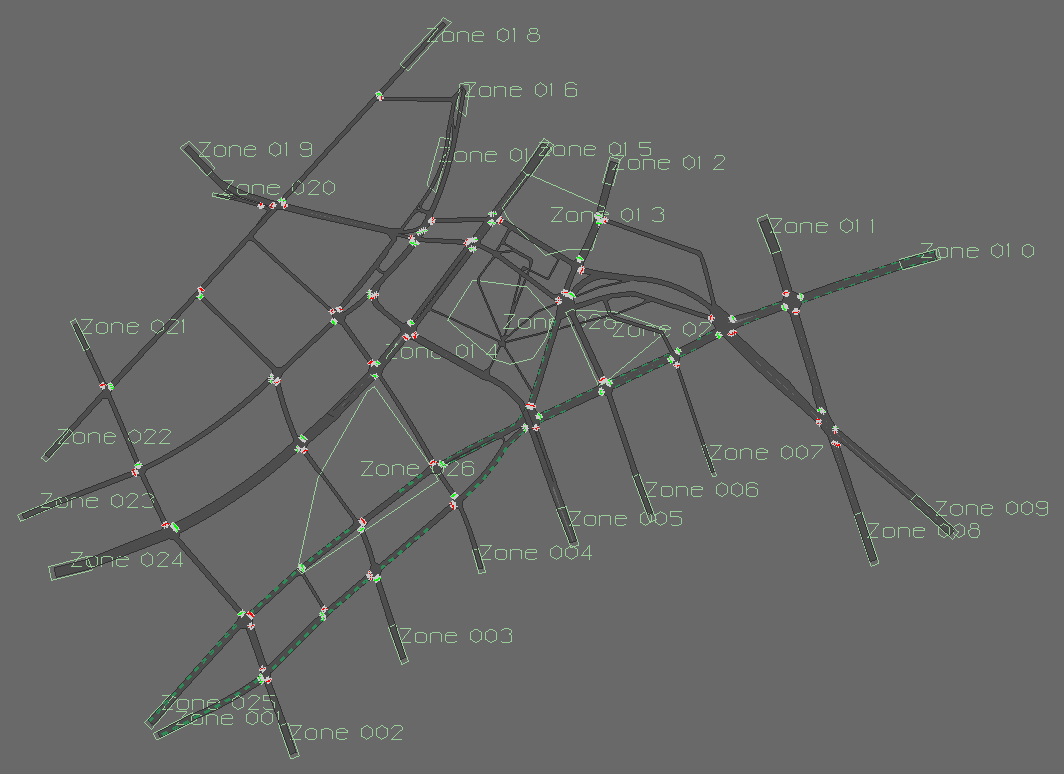
\includegraphics[width=\linewidth]{figuras/costanera.png}
        \caption{Mapa en Paramics del escenario simulado.}
    \end{subfigure}\\
    \begin{subfigure}{0.8\textwidth}
        \centering
        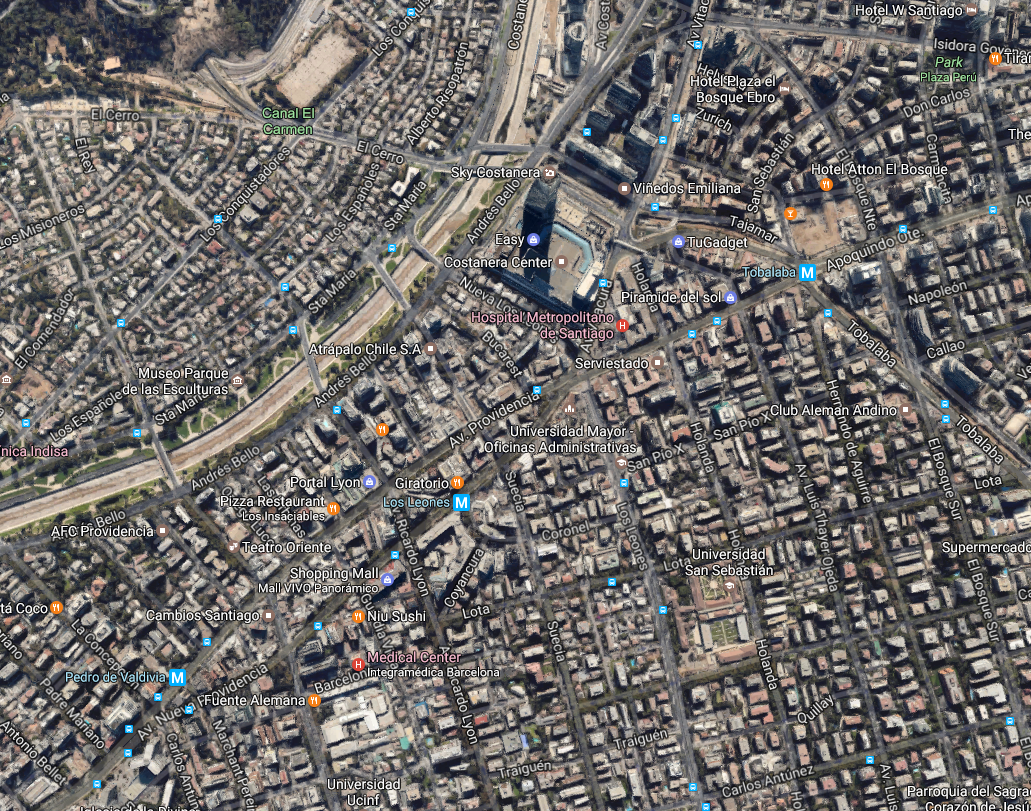
\includegraphics[width=\linewidth]{figuras/costanera_maps.png}
        \caption{Escenario simulado en la ``vida real'', Google Maps.}
    \end{subfigure}
    \caption{Escenario modelado, Paramics vs. ``vida real''.}
    \label{fig:costanera}
\end{figure}

Como escenario de transporte para la validación del \emph{framework} se utilizó un modelo de un sector de la ciudad de Santiago de Chile, el cual consiste en una simulación detallada del flujo vehicular en la comuna de Providencia. Este modelo fue creado en 2010 por Víctor Zúñiga para el desarrollo de su memoria de grado \autocite{zuniga}, y simula el impacto sobre el sector entre las avenidas Providencia, Tobalaba, Andrés Bello y Santa María proyectado en ese entonces por la construcción de un nuevo centro comercial (ver figura \ref{fig:costanera}).

Sobre este escenario vehicular se construyó un modelo de ITS, utilizando el \emph{plugin} desarrollado y el \emph{framework} VEINS en OMNeT++. Este consistió en un escenario en que un vehículo sufre un desperfecto en una cierta calle de la simulación y emite \emph{beacons} de advertencia en \emph{broadcast} a todos los demás vehículos que se encuentran dentro del alcance de la transmisión. A aquellos vehículos que reciben un \emph{beacon}, y que se puede predecir ingresarán a a la calle en que se encuentra el vehículo averiado, se les modifica luego su ruta mediante VEINS y TraCI.

De manera más detallada, el escenario funciona de la siguiente manera:

\begin{enumerate}
    \item Al iniciarse el \emph{framework}, OMNeT++ (utilizando VEINS) inicializa una conexión TraCI con el \emph{plugin} en Paramics.
    \item Por cada vehículo que ingresa a la red de transporte, OMNeT++ crea un módulo dotado de lógica y capacidades comunicaciones en su simulación de red, y asocia el movimiento de este módulo al vehículo en Paramics. En adelante, se entenderá por ``vehículo'' el par consistente en el vehículo en Paramics y su módulo asociado en OMNeT++.
    \item Periódicamente se verifica la posición de cada vehículo, y al detectar el primero en ingresar a la calle del ``accidente'', este es detenido. La calle en cuestión para esta simulación fue el arco ``40:5'', el cual corresponde a Avenida Vitacura, frente al centro comercial. El vehículo además se colorea rojo para su fácil identificación.
    \item El módulo OMNeT++ del vehículo accidentado emite luego, cada 5 segundos, un mensaje WAVE \autocite{80211wave} en \emph{broadcast}.
    \item Aquellos vehículos que reciban el \emph{beacon} de emergencia, se encuentren en alguna de las calles aledañas al accidente y que tengan un destino que probablemente los haga pasar por la calle afectada, cambian su ruta a utilizar el arco ``40:7'', correspondiente a la calle Holanda, entre Avda. Vitacura y Avda. Providencia. Además, se cambia su color a púrpura para visualizarlos de manera más fácil en Paramics.
\end{enumerate}

Esta simulación dura un total de \textbf{15 minutos de tiempo \emph{simulado}}, y se ejecutó con múltiples configuraciones del sistema de transporte y del sistema de comunicaciones, las cuales se verán a continuación en la sección \ref{sec:measurements}.

Finalmente, estas simulaciones se realizaron en un equipo cuyas especificaciones técnicas pueden observarse en la tabla \ref{table:systemspecs}.

\begin{table}[tpb]
    \centering
    \begin{tabular}{@{}ll@{}}
        \toprule
        Sistema Operativo     & Windows 10 v.10.0.14393         \\
        Procesador            & Intel Core i7 4720HQ @ 2.60 GHz \\
        N$^{o}$ de Núcleos / Threads & 4 núcleos / 8 threads\\
        Arquitectura          & x86\_64                         \\
        RAM                   & 12 GB DDR3L 1600 MHz            \\
        Tarjeta de Video      & NVIDIA GeForce GTX 960M         \\
        Memoria Video         & 2 GB GDDR5                      \\ \bottomrule
    \end{tabular}
    \caption{Especificaciones técnicas del entorno de simulación.}
    \label{table:systemspecs}
\end{table}

\subsection{Mediciones realizadas} \label{sec:measurements}

Las mediciones realizadas se enfocaron a probar el funcionamiento del \emph{framework} en dos categorías de análisis; \textbf{eficiencia computacional} de la implementación e \textbf{impacto sobre el modelo de transporte}. De esta manera se pretende demostrar que PVEINS es una opción viable para la investigación en Sistemas Inteligentes de Transporte, tanto en términos de los recursos que utiliza el \emph{framework} para la ejecución de las simulaciones como en términos de la validez de los resultados obtenidos.

\subsubsection{Eficiencia computacional}

\begin{table}[tpb]
    \centering
    \begin{tabular}{@{}rrr@{}}
        \textbf{Factor de Demanda} & \textbf{Ctdad. Prom. Vehículos} \\ \midrule
        100\%           & 1379.9 \\ %\midrule
        75\%            & 868.75 \\ %\midrule
        50\%            & 514.5825 \\ %\midrule
        25\%            & 246.5675 \\ \bottomrule
    \end{tabular}
    \caption[Factor de demanda vs. cantidad promedio de vehículos]{Tabla de relación entre factor de demanda y cantidad promedio de vehículos por instante de tiempo en el escenario de prueba.}
    \label{table:demandfactor}
\end{table}

El principal factor a medir en esta categoría es la relación entre la cantidad de vehículos en una simulación y el tiempo real que demora el \emph{framework} en simular el escenario, para una duración en tiempo simulado específica. De esta manera, se pretende caracterizar el comportamiento del \emph{software} para escenarios vehiculares de alta complejidad, en los cuales pueden llegar a interactuar miles de vehículos. Además, interesa también la carga en términos de recursos de sistema que genera la ejecución de la simulación sobre el equipo de prueba. 

A través de éstos datos se pretende generar un perfil del \emph{software} que indique los requisitos que impone sobre el entorno de simulación, y su factibilidad de uso para sistemas de transporte complejos tanto en entornos de simulación de alto rendimiento como de mediano y bajo.

Antes de detallar las simulaciones realizadas, se debe definir el término \emph{factor de demanda}. Éste corresponde a un elemento de configuración de la simulación de transporte en Paramics, el cual caracteriza la carga vehicular sobre el sistema de transporte en cada instante de tiempo. En términos más simples, el factor de demanda regula la cantidad de vehículos que Paramics inserta a la red durante la simulación; es un valor porcentual cuya correspondencia en cantidad real de vehículos en la red dependerá de las características particulares de cada simulación. Sin embargo, los valores aproximados para el escenario utilizado, para distintos factores de demanda, pueden observarse en la tabla \ref{table:demandfactor}.

Se realizaron entonces 16 ejecuciones del escenario (de aquí en adelante, denominadas \emph{runs}) con cuatro factores de demanda distintos (4 \emph{runs} con 100\%, 4 con 75\%, 4 con 50\% y 4 con 25\%) y cada una con una \emph{semilla} distinta para los generadores de números pseudoaleatorios. De éstos \emph{runs} se extrajeron las siguientes estadísticas:

\begin{enumerate}
    \item Timestamp de inicio del \emph{run}.
    \item Timestamp de fin del \emph{run}.
    \item Duración en tiempo real del \emph{run}.
    \item Cantidad de vehículos en la red de transporte, cada 1 minuto de tiempo simulado.
\end{enumerate}

Además, se realizó una ejecución adicional de un \emph{run} con factor de demanda 100\%, y se midió la carga sobre el equipo de prueba mientras se ejecutaba la simulación utilizando las herramientas de monitoreo de sistema de Microsoft Windows. En específico, se midió la carga porcentual sobre el procesador, la memoria RAM utilizada y la cantidad de operaciones de escritura y lectura del disco físico durante la simulación. 

\subsubsection{Impacto sobre el modelo de transporte}

